\chapter{Implementation}
\label{chapter:implementation}
% This chapter should describe what was actually produced: the programs which were written, the hardware which was built or the theory which was developed. Any design strategies that looked ahead to the testing stage might profitably be referred to (the professional approach again).
% Descriptions of programs may include fragments of high-level code but large chunks of code are usually best left to appendices or omitted altogether. Analogous advice applies to circuit diagrams.
% Draw attention to the parts of the work which are not your own. The Implementation Chapter should include a section labelled ”Repository Overview”. The repository overview should be around one page in length and should describe the high-level structure of the source code found in your source code Repository. It should describe whether the code was written from scratch or if it built on an existing project or tutorial. Making effective use of powerful tools and pre-existing code is often laudable, and will count to your credit if properly reported.
% It should not be necessary to give a day-by-day account of the progress of the work but major milestones may sometimes be highlighted with advantage.

%  ~4,500 words

% Tangent works better than correlation or partial correlation.
\section{Overview}

\begin{figure}[]
    \centering
    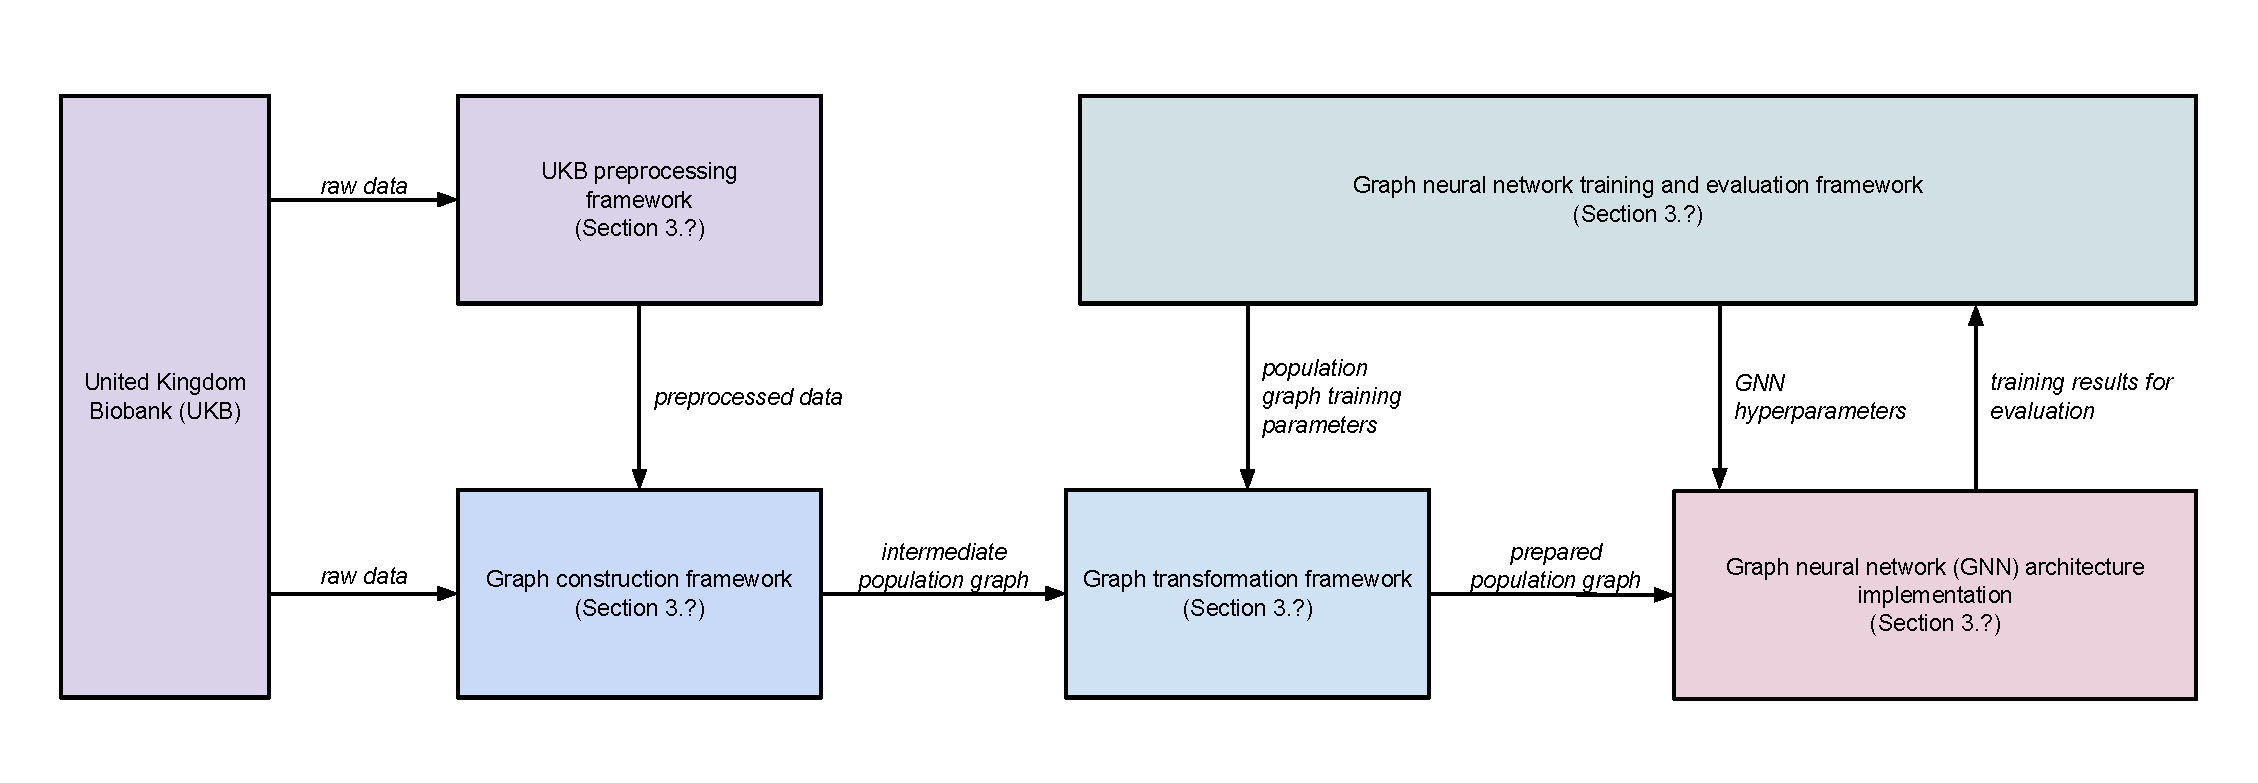
\includegraphics[width=\textwidth]{pipeline_overview.pdf}
    \caption{Overview of the key project components.}\label{pipeline-overview}
\end{figure}

This project can be divided into five key components, as illustrated in Figure~\ref{pipeline-overview}:
\begin{enumerate}
    \item Preparation of the United Kingdom Biobank (UKB) dataset;
    \item Intermediate population graph construction;
    \item Population graph transformation for training;
    \item Training on graph neural network architectures;
    \item Evaluation of the graph neural network performance.
\end{enumerate}

The work was split into these particular components so that each of them can carry out a single task independently of the other parts of the program (other than the clearly defined input/output communication), following requirement R3 (see Section~\ref{section:requirements-analysis}). This makes the overall project easier to implement, understand and extend in the future, generalising it to other datasets and preprocessing methods. 

This chapter will explain in detail the implementation behind each of the components.

\section{UKB preprocessing component}
\label{section:ukb-preprocessing}

The main function of the UKB preprocessing component is to prepare the raw or partially preprocessed UKB data for population graph construction. In particular, to improve the computational efficiency of operations later in the pipeline (potentially saving hours or days of computation time), this component preprocesses the data in a convenient form. This involves filtering the dataset, precomputing similarity matrices and functional connectivity matrices. The schematic diagram of these steps is shown in Figure~\ref{preprocessing-component}, which will be referred to throughout this section.

\begin{figure}[h]
    \centering
    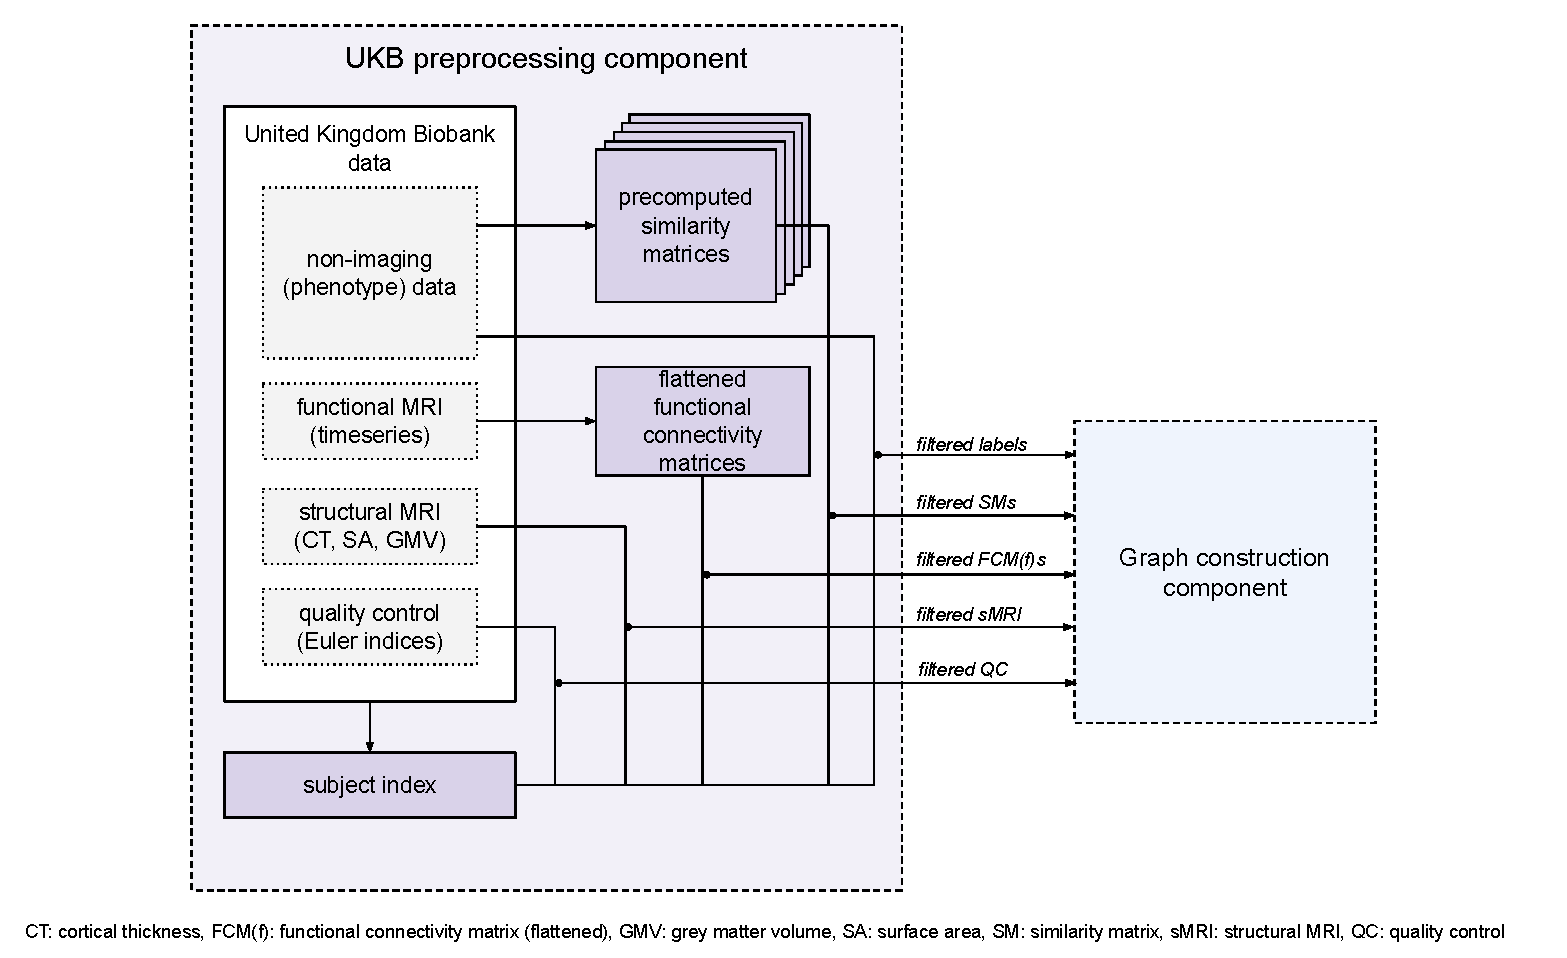
\includegraphics[width=\textwidth]{preprocessing_component.pdf}
    \caption{Overview of the UKB preprocessing component.}\label{preprocessing-component}
\end{figure}

\subsection{Cleaning the dataset}
The different modalities of the UKB data, shown in the white box in Figure~\ref{preprocessing-component}, have been provided separately from each other, with a small minority of subjects having the data available for some of the modalities but not others (for example, due to data corruption or its retraction by the participant). To ensure consistent and smooth processing, the subjects with partially missing data (236 in total) have been excluded from further processing. The remaining 17,314 subjects with well-defined modalities have been collected into a \textit{subject index} (bottom left of Figure~\ref{preprocessing-component}), which was used to select, filter and index the data in the subsequent components of the pipeline.

% TODO rb643: as mentioned in another comment I think in future we can do a bit more data cleaning and include additional features in your similarity computation
% TODO rb643: In future implementations it may be worth considering either cortex only or split matrices for cortical and subcortical

\subsection{Precomputing connectivity matrices}
The connectivity matrices involve computing pairwise correlations of 376 time-series (for 360 cortical and 16 subcortical regions) for every subject. With 20 gigabytes of raw time-series data across over 17,000 subjects, this introduces a high computational overhead (a few hours on a CPU\footnote{Measured on a Computational Biology lab machine.} per population graph) if the matrices have to be recomputed every time the graph is constructed. To avoid this, the matrices are computed once for every subject, flattened and their lower triangles stored as \texttt{numpy} arrays as part of the preprocessing component.

% could include the maths here?

\subsection{Precomputing similarity matrices}
The computation of pairwise similarity scores is quadratic in both time and space with respect to the number of subjects. Depending on the exact method of how the similarity function is computed, a general-purpose (non-accelerated) processor might take hours or even days to process the entire dataset. The repeated computation would also be wasteful, since the similarities for a single non-imaging feature do not change over different population graphs: the variation comes from different \textit{selections} of subjects and non-imaging features, their relative weighting, and similarity thresholds.

The similarity matrices – one for each non-imaging feature in Table~\ref{table:phenotype-features} – have therefore been computed in advance. Unlike the functional connectivity data that is used directly for population graph node features (and is flattened and reduced to avoid redundancy), the feature-wise similarity matrices are sliced and filtered depending on the selection of subjects. In this case, it is more practical to store the full matrix, so that the integer indices into the similarity matrix directly correspond to the subject index in other components of the population graph data structure (see Sections~\ref{section:ukb-preprocessing} and~\ref{section:population-graph-representation}).

Having computed the feature-wise similarity matrices, their linear combination for a full similarity score (by default adding matrices together and dividing the result by a constant) can efficiently make use of vectorised matrix operations.

For the \texttt{ICD10} metric, the subjects were considered to be \texttt{ICD10}-similar whenever they had at least one shared mental health or nervous system diagnosis. Two patients without any mental health or nervous system diagnoses were \textit{not} considered to be similar, however, since similarity in having a healthy brain is extremely common (thus not in itself informative) while causing memory issues (see Section~\ref{section:memory}). 

The similarity computation was vectorised in order to make use of hardware acceleration and reduce the compute time: for the boolean \texttt{ICD10}-lookup matrix $\mathbf{F}_{\text{ICD10}}$ with rows indexed by subjects and columns by relevant \texttt{ICD10} diagnoses, the pairwise similarity matrix $\mathbf{M}_{\text{ICD10}}$ computation corresponds to 

\begin{equation}
    \mathbf{M}_{\text{ICD10}} = \mathbf{1}\left[\mathbf{F}_{\text{ICD10}}^{\ }\mathbf{F}_{\text{ICD10}}^{\mathrm{T}} \geq 1\right]
\end{equation}

with the indicator function $\mathbf{1}[\cdot]$ applied element-wise.

For the remaining metrics (e.g.\ years of full-time education, \texttt{FTE}) there is only one integer or floating-point value per subject, with values  compared for equality. The computation is vectorised by exploiting tensor broadcasting semantics\footnote{\url{https://pytorch.org/docs/stable/notes/broadcasting.html}} that copy rows and columns as necessary for the matrix dimensions to match. For the vector of subject \texttt{FTE}s, $\mathbf{f}_{\text{FTE}}^{\mathrm{T}} \in \mathbb{R}^{N \times 1}$ and $\mathbf{F}_{\text{FTE}} = [\mathbf{f}_{\text{FTE}}^{\mathrm{T}} \cdots \mathbf{f}_{\text{FTE}}^{\mathrm{T}}] \in \mathbb{R}^{N \times N}$, \texttt{FTE}-similarity matrix is defined as

\begin{equation}
    \mathbf{M}_{\text{FTE}} = \mathbf{1}\left[\mathbf{F}_{\text{FTE}}^{\ } = \mathbf{F}_{\text{FTE}}^{\mathrm{T}} \right].
\end{equation}


% \[
% \begin{blockarray}{rccccc}
%  & b & c & d & e & f \\
% \begin{block}{r[ccccc]}
%   \text{UKB} & 1 & 1 & 1 & 1 & f \\
%   0 & 1 & 0 & 0 & 1 & g \\
%   0 & 0 & 1 & 0 & 1 & h \\
%   0 & 0 & 0 & 1 & 1 & i \\
%   0 & 0 & 0 & 0 & 1 & j \\
% \end{block}
% \end{blockarray}
%  \]

\section{Graph construction component}
\label{section:graph-construction}
The next stage of the pipeline involves constructing the ``intermediate representation'' of the population graph. The intermediate representation contains the graph topology and node features, but is not prepared for training – it is not split into training, validation and test sets, and its features are not normalised. The two stages are separate because this allows for the reuse of the same intermediate representation for different dataset splits and other training parameters without having to reconstruct the edges in $O(N^2)$ time for $N$ subjects. The steps for the data processing in this component are schematically visualised in Figure~\ref{graph-construction-component}.

\begin{figure}[h]
    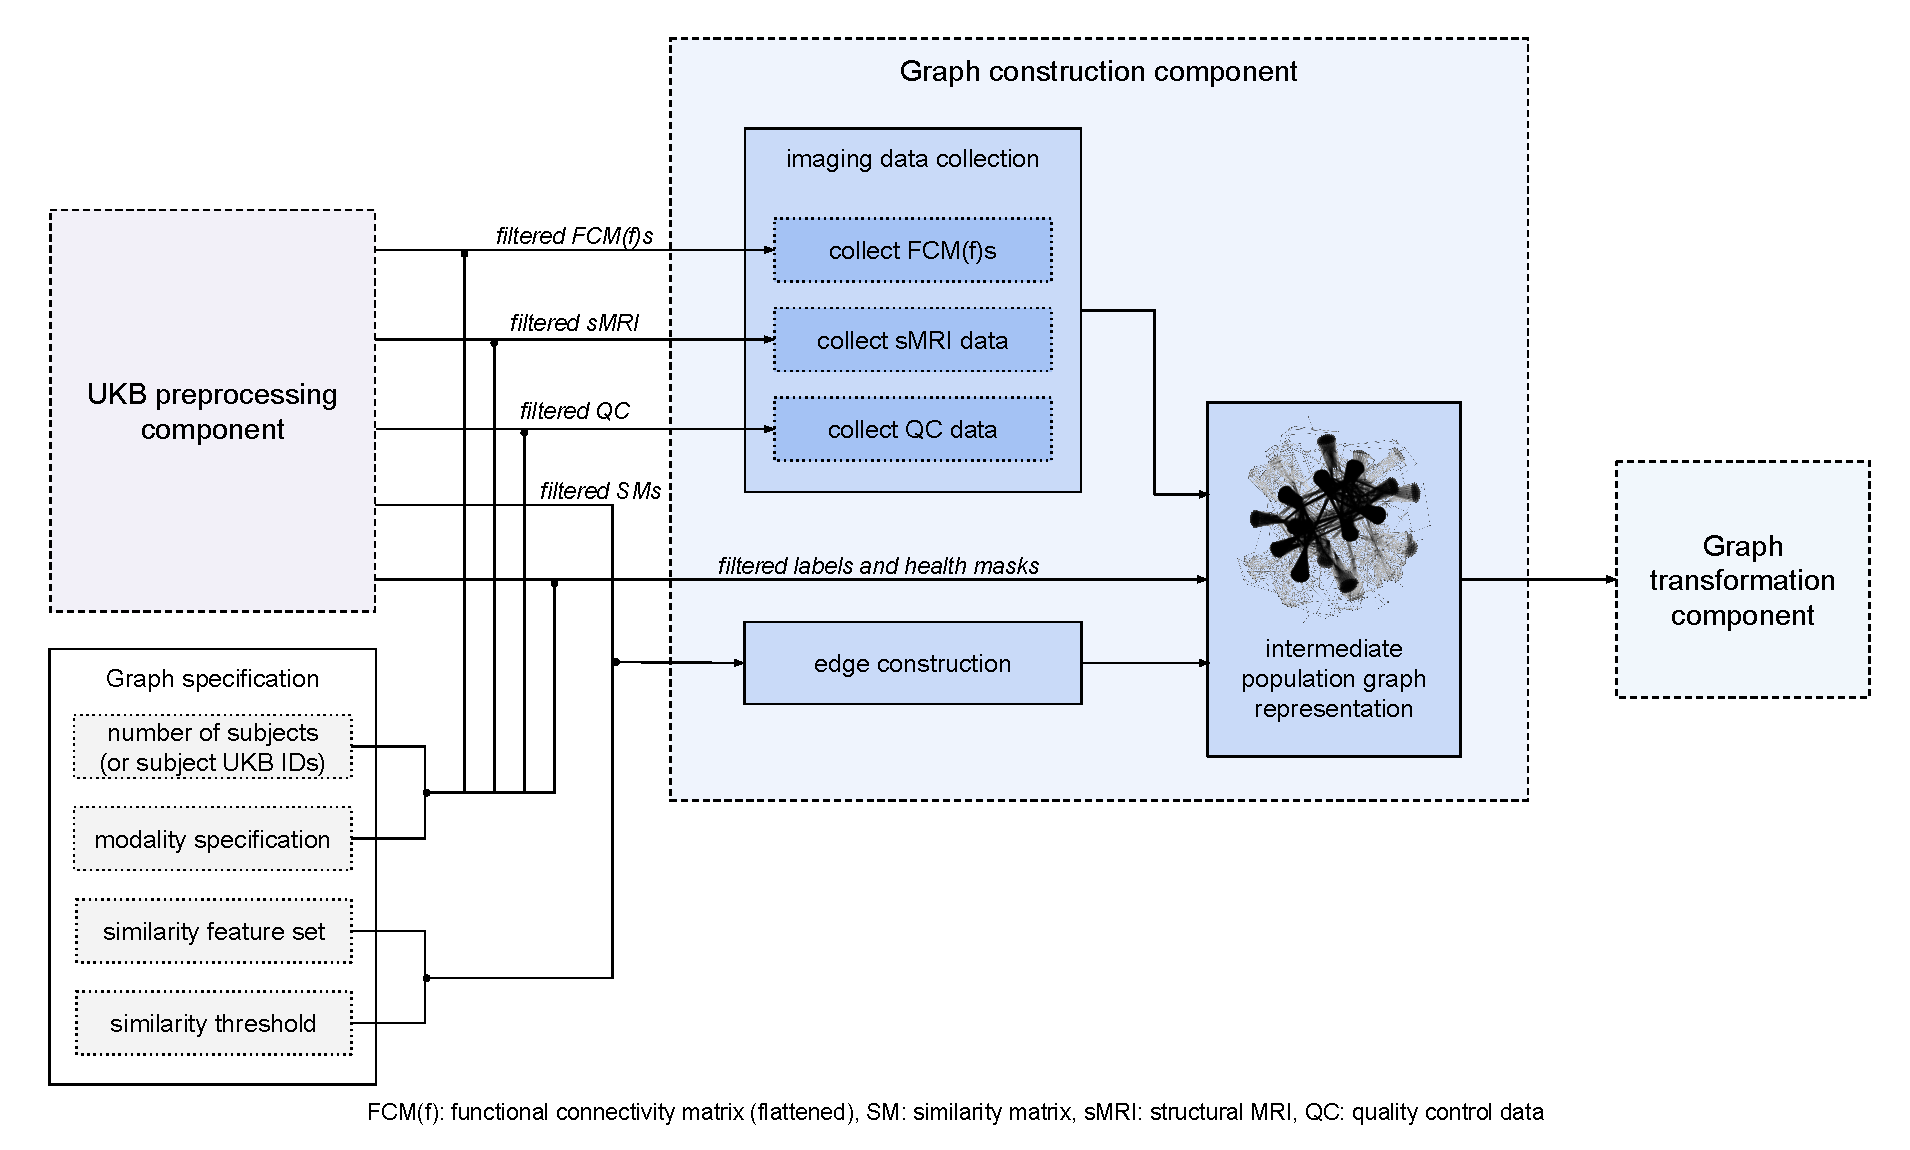
\includegraphics[width=\textwidth]{graph_construction_component.pdf}
    \caption{Graph construction component.}\label{graph-construction-component}
\end{figure}

\subsection{Inputs}
The inputs to the graph construction component can be categorised into four types as shown in the box at the bottom left of Figure~\ref{graph-construction-component}:
\begin{enumerate}
    \item \textit{Modality specification} describes which of the neuroimaging modalities should be used as node features. This could be any combination of functional, structural and quality control data, following the pipeline flexibility requirement R2 (Section~\ref{section:requirements-analysis}).
    \item \textit{Subject specification} is an optional argument overriding the default option to use the entire dataset (filtered by the subject index described in the previous component) when constructing the population graph. In this case, a number of subjects or a list of particular UKB identifiers could be provided.
    \item \textit{Similarity specification}. 
    In its default implementation, the similarity score is computed as the average over a set of similarity features $\{M_1, \dots, M_n\}$ (see Equation~\eqref{eq:similarity}), in which case it is sufficient to specify the similarity feature set to be used. An extension to this is to accept an arbitrary linear combination of various similarity features, allowing for much richer similarity metrics, again increasing the flexibility of the pipeline (see Requirement R2 in Section~\ref{section:requirements-analysis}). 
    \item \textit{Similarity threshold}. A number $\mu \in [0,1]$ defining the threshold for the similarity metric above which an edge will be added to the graph (see Equation~\eqref{eq:similarity-threshold}).
\end{enumerate}


\subsection{Imaging data collection}

Based on the subject and modality specification, the relevant imaging data is collected from the raw UKB files (first filtered by subject index) and stored in the intermediate representation as a \textit{dataframe} (\texttt{pandas.DataFrame} object) indexed by UKB subject identifier. This is represented by the connections between UKB preprocessing component, graph specification and the blue imaging data collection box in Figure~\ref{graph-construction-component}. 

If a particular modality is unused, the dataframe stored is empty.

\subsection{Edge construction}

The edge construction component uses the similarity specification and the filtered similarity matrix data to find the similarity scores for each pair of subjects determined by the subject specification. Whenever the similarity score between two subjects exceeds the threshold, an undirected edge is added to the population graph. The edges are stored in a \textit{tensor} (\texttt{torch.tensor}), a PyTorch datatype for multi-dimensional matrices\footnote{\url{https://pytorch.org/docs/stable/tensors.html}}.

\subsection{Brain health mask computation}

Following the brain age estimation method discussed in Section~\ref{brain-age-estimation}, the machine learning model can only be trained on subjects with healthy brains, although the population graph may contain both healthy and non-healthy subjects. The \textit{brain health mask} is therefore computed to determine which subjects can be used to train the model and which cannot. In particular, non-healthy subjects are not included in loss function computation, so that the direction of parameter update depends on healthy subjects only (though the parameters are updated for the entire graph). As a result, the age predictions are available for both healthy and non-healthy subjects, but the use of a brain health mask ensures that the prediction corresponds to the brain age rather than chronological age, as discussed in Section~\ref{brain-age-estimation}.

In this project, the brain health is approximated by the absence of diagnoses related to mental health or nervous system disorders, defined by the \texttt{ICD10}-similarity metric (see Table~\ref{table:phenotype-features}).

\subsection{Population graph representation}
\label{section:population-graph-representation}

The population graph is stored in an extended \texttt{torch\_geometric.Data} object\footnote{\url{https://pytorch-geometric.readthedocs.io/en/latest/modules/data.html}}, with its most important fields listed in Table~\ref{table:population-graph}. The intermediate population graph representation has all its entries defined except for the feature vector \texttt{x} and the training, validation and test masks.

\setlength{\LTpost}{0pt}
\renewcommand{\arraystretch}{1.25}
% \begin{table}[]
%     \caption{The population graph data structure (excludes helper or utility fields).}\label{table:population-graph}
%     \centering
%     \begin{tabular}{lp{0.2\textwidth}p{0.5\textwidth}}
%         \hline
\begin{center}
\begin{longtable}[]{lp{0.175\textwidth}p{0.475\textwidth}}
    \caption{The population graph data structure (excludes helper or utility fields).}\label{table:population-graph}\\
    \hline \textbf{Field name} & \textbf{Type} & \textbf{Description} \\
    \hline
    \endfirsthead
    \multicolumn{3}{c}%
    {\tablename\ \thetable\ -- \textit{Continued from previous page}} \\
    \hline
    \textbf{Field name} & \textbf{Type} & \textbf{Description} \\
    \hline
    \endhead
    \hline \multicolumn{3}{r}{\textit{Continued on next page}} \\
    \endfoot
    \hline
    \endlastfoot
    % \texttt{num\_nodes} & long & Number of nodes (subjects) in the population graph. \\
    \texttt{subject\_index} & string array & UKB identifiers of the subjects. Stored in the same subject order as training masks, feature and label tensors; corresponds to the edge start and end values. \\
    \texttt{edge\_index} & $2\times 2|E|$ \hfill\newline long tensor & \texttt{edge\_index}$[0][i]=s_v$ and \hfill \newline \texttt{edge\_index}$[1][i]=s_w$ indicate a directed \hfill \newline edge $s_v \leadsto s_w$. Following the PyTorch Geometric API, to represent the undirected edge $(s_v, s_w) \in E$, another directed edge $s_w \leadsto s_v$ is added. \\
    \texttt{functional\_data} & dataframe & Row-indexed by subject with columns containing the flattened functional connectivity matrix entries. Empty if no functional data is used in the population graph. \\
    \texttt{structural\_data} & dictionary of \hfill \newline dataframes & Dictionary is indexed by the structural data modality, in this case cortical thickness, surface area, and grey matter volume. The corresponding dataframes are row-indexed by subject with columns containing the features of the relevant structural data modality. The dataframes are empty if no structural data is used. \\
    \texttt{quality\_control\_data} & dataframe & Row-indexed by subject with two columns containing Euler indices for the left and right hemispheres of the brain. Empty if no quality control data is used. \\
    \texttt{x} & $N \times F$ \hfill\newline float tensor & \textit{Unused at the intermediate stage.} Contains the full normalised feature vector (of $F$ features) for every graph node (subject). \\
    \texttt{y} & $N \times 1$ \hfill \newline float tensor & Contains the labels of training data, in this case chronological age. \\
    \texttt{brain\_health\_mask} & boolean array & \texttt{True} indicates that the subject has a healthy brain and can be used for training, and \texttt{False} otherwise. \\
    \texttt{train\_mask} & boolean tensor & \textit{Unused at the intermediate stage.} \texttt{True} if the subject belongs to the training set, and \texttt{False} otherwise. \\
    \texttt{validation\_mask} & boolean tensor & \textit{Unused at the intermediate stage.} \texttt{True} if the subject belongs to the validation set, and \texttt{False} otherwise. \\
    \texttt{test\_mask} & boolean tensor & \textit{Unused at the intermediate stage.} \texttt{True} if the subject belongs to the test set, and \texttt{False} otherwise.
    % \end{tabular}
\end{longtable}
\end{center}

\subsection{Testing}
As discussed in requirement R1 for this project (see Section~\ref{section:requirements-analysis}), it is important to ensure that the data is preprocessed and collected into the population graph correctly. To this end, both the UKB preprocessing (Section~\ref{section:ukb-preprocessing}) and the graph construction components have unit test modules asserting the correctness of the similarity matrices and example graph topologies.

\section{Graph transformation component}
\label{section:graph-transformation}

The graph transformation component is responsible for preparing the intermediate population graph representation for training by defining its normalised, concatenated feature vector as well as training, validation and test masks, using the parameters provided by the training component. The schematic diagram representing the population graph transformations in this component is shown in Figure~\ref{graph-transformation-component}.

\begin{figure}[h]
    \centering
    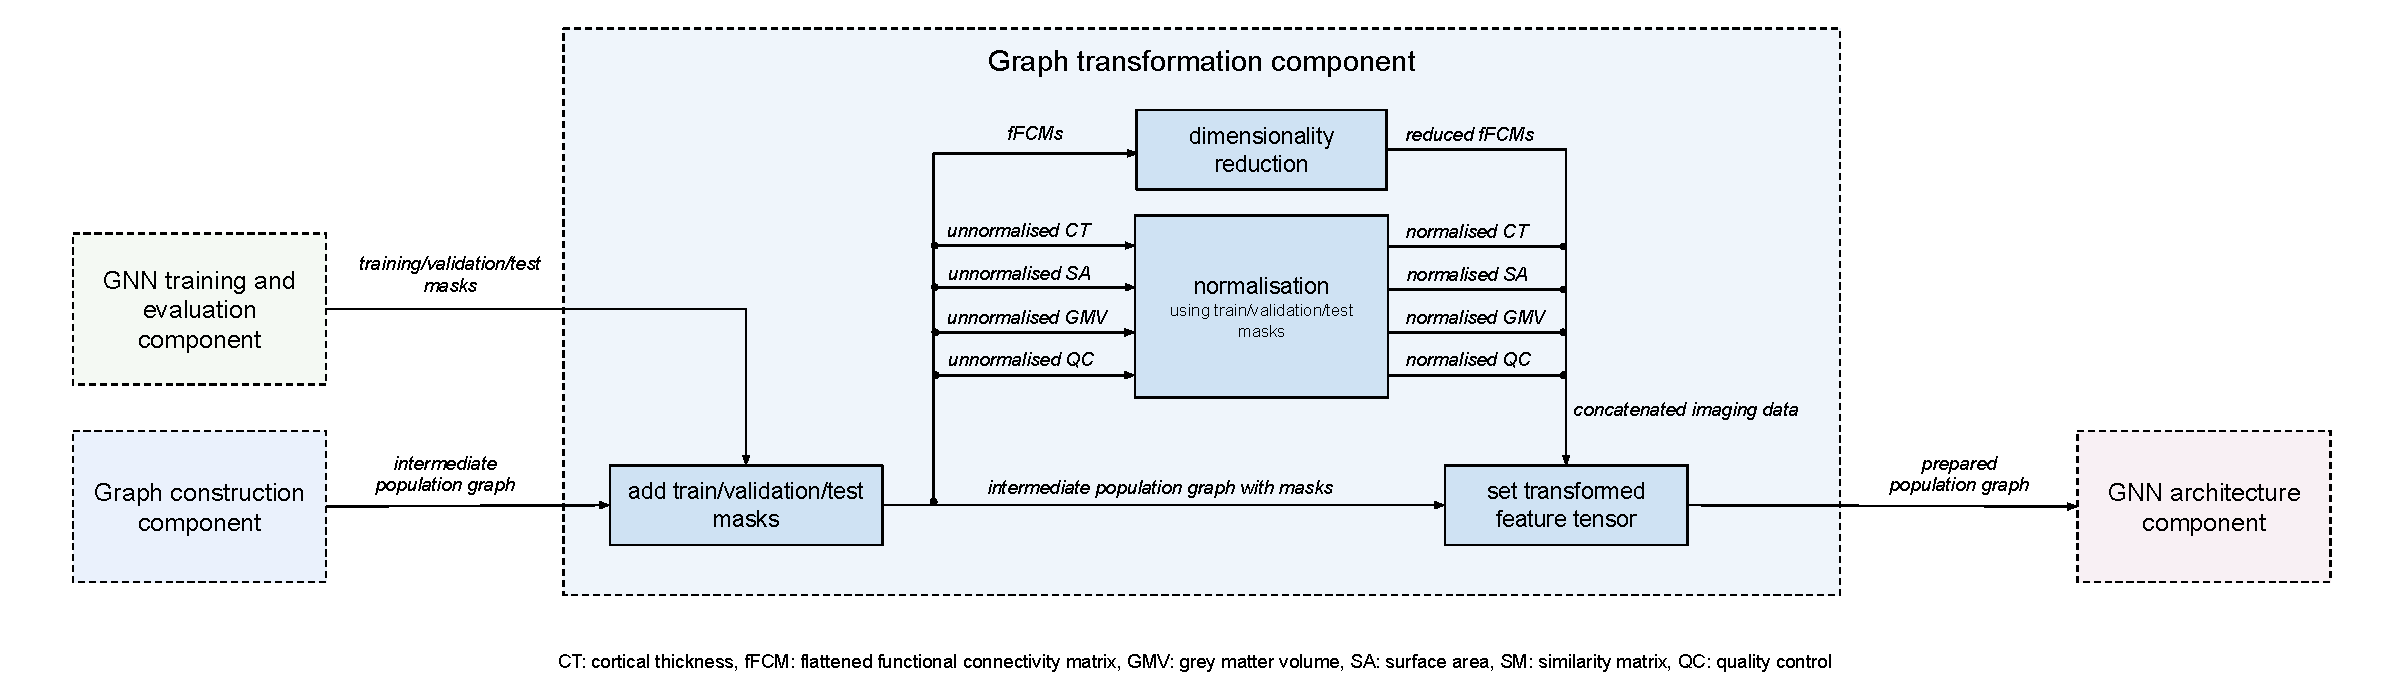
\includegraphics[width=\textwidth]{graph_transformation_component.pdf}
    \caption{Graph transformation component.}\label{graph-transformation-component}
\end{figure}

\subsection{Setting the training masks}
\label{setting-training-masks}
The first operation for preparing the population graph for training involves setting the \texttt{train\_mask}, \texttt{validation\_mask} and \texttt{test\_mask} fields of the intermediate population graph data structure (see Table~\ref{table:population-graph}). The masks are defined in the GNN training and evaluation component as this depends on the training procedure, not the structure of the population graph itself.

Following the brain age estimation method (Section~\ref{brain-age-estimation}), the masks are intersected with the \texttt{brain\_health\_mask}. Similarly to the function of the brain health mask, the three training masks are used to determine which nodes should be used to compute the loss function during various stages of training. For example, the model parameters are only updated based on the loss function for the subjects filtered with the \texttt{training\_mask}, and validation loss is computed only for the subjects filtered with the \texttt{validation\_mask}.

% TODO rb643: Again more for future implementation: I've been playing around with running PCA on the raw time-series as well as Diffusion Embedding on the connectivity matrices and they provide strikingly similar results. Thus is might be computationally efficient to use raw time-series PCA in the future. Generally only the first half dozen PC's are interesting anyway
\subsection{Functional connectivity matrix dimensionality reduction}
The flattened functional connectivity matrix results in over 70,000 features per patient. Since the population graph cannot be split into parts and during training must be kept entirely in memory, along with all model parameters, this quickly runs into memory issues when the entire dataset is used. To mitigate this issue, some techniques may be applied to reduce the dimensionality of functional data. This project uses principal component analysis (PCA) as the dimensionality reduction technique of choice as it is one the simplest to implement. When the functional data is used to construct the population graph, PCA transformation is fitted to the training set as specified by the \texttt{training\_mask}, and the same transformation is applied to the remaining subjects. This dimensionality reduction technique is optional in the pipeline, and it is possible to define how many principal components should be kept after the transformation to control the information loss. By default, only 1\% of the most important components are kept so that the number of functional and structural features have the same order of magnitude.

\subsection{Structural MRI and quality control data normalisation}
Next, the raw features stored under \texttt{structural\_data} and \texttt{quality\_control\_data} are normalised to be in the range between $-1$ and $1$ with mean 0. Similar to the previous section, in order to avoid data leakage a standard scaler is fitted to the training set only (as specified by the \texttt{training\_mask}) and then applied to the validation and test sets. A separate transformation is applied to each structural data modality (cortical thickness, surface area, grey matter volume) and the quality control modality.

\subsection{Setting the transformed feature tensor}
The transformed functional, structural and quality control features are concatenated together into a single tensor, which is assigned to \texttt{x} in the population graph data structure (Table~\ref{table:population-graph}). This completes graph transformation for training.

Since the original neuroimaging dataframes and brain health masks are kept unchanged in the data structure, the same population graph can be prepared for, say, a different training fold by simply going through the transformation component again but with a different training mask set, which will reset the values in the corresponding population graph fields. This explains the communication loop between the graph transformation and GNN training and evaluation components in Figure~\ref{graph-transformation-component}.

\section{GNN architecture component}
\label{section:gnn-architecture}
% gcn_train(graph, device, n_conv_layers=0, layer_sizes=None, epochs=3500, lr=0.005, dropout_p=0, weight_decay=1e-5,
% log=True, early_stopping=True, patience=10, delta=0.005, cv=False, fold=0, run_name=None,
% min_epochs=1000):

The graph neural network component contains implementations for the graph neural network (GNN) architectures used in this project: the graph convolutional network (GCN, Section~\ref{training-gcn}) and the graph attention network (GAT, Section~\ref{training-gat}). The networks are implemented as two PyTorch modules called \texttt{BrainGCN} and \texttt{BrainGAT}, extending a shared \texttt{BrainGNN} module. Table~\ref{table:braingnn} presents the parameters used to define a \texttt{BrainGNN} instance. Then instantiating \texttt{BrainGCN} and \texttt{BrainGAT} simply amounts to setting the \texttt{conv\_type} parameter to either \texttt{GCN} or \texttt{GAT}, and setting the convolutional layers to either \texttt{torch\_geometric.nn.GCNConv} or \texttt{torch\_geometric.nn.GATConv} respectively, reusing the rest of the code. The implementations for \texttt{GCNConv} and \texttt{GATConv} are available in the PyTorch Geometric library.


\begin{center}
    \begin{longtable}[]{p{0.275\textwidth}p{0.175\textwidth}p{0.475\textwidth}}
        \caption{The parameters for the \texttt{BrainGNN} module.}\label{table:braingnn}\\
        \hline \textbf{Parameter} & \textbf{Type} & \textbf{Description} \\
        \hline
        \endfirsthead
        \multicolumn{3}{c}%
        {\tablename\ \thetable\ -- \textit{Continued from previous page}} \\
        \hline
        \textbf{Parameter} & \textbf{Type} & \textbf{Description} \\
        \hline
        \endhead
        \hline \multicolumn{3}{r}{\textit{Continued on next page}} \\
        \endfoot
        \hline
        \endlastfoot
        
        \texttt{conv\_type} & string & Indicates the type of graph convolutional layer to be used (graph convolution or graph attentional layer). \\
        \texttt{layer\_sizes} & integer array & Lists the number of units in every hidden layer. The length of the array corresponds to the total number of hidden layers. \\
        \texttt{n\_conv\_layers} & integer & Number of convolutional layers. Must be in range $[0, \text{\texttt{len(layer\_sizes})}]$. The sizes of those layers are determined by the first \texttt{n\_conv\_layers} values of the \texttt{layer\_sizes} and \texttt{n\_node\_features} parameters. \\
        \texttt{num\_node\_features} & integer & Indicates the number of input features. \\ 
        \texttt{dropout\_p} & float $\in [0,1]$& The probability of ignoring the node in a hidden layer at training time. Used as a regularisation technique to reduce overfitting.
    \end{longtable}
    \end{center}

Listing~\ref{listing:braingnn} shows how the layers are combined in the \texttt{BrainGNN} architecture for a given set of parameters in Table~\ref{table:braingnn}. Hyperbolic tangent ($\tanh(\cdot)$) was chosen as the non-linearity (activation function) between each layer. This is because the population graph features and weights in neurons may be negative, in which case other popular activation functions such as $\mathrm{ReLU}(\cdot)$ may have an undesirable asymmetric response.

The \textit{dropout} (\texttt{torch.nn.Dropout}) layers have been added between the every fully connected layer in line 21 as a \textit{regularisation} technique to avoid overfitting. With probability \texttt{dropout\_p}, a unit in the layer is ignored at training time (its weight is zeroed) with the goal that the neural network does not rely on any particular neuron when predicting age, therefore learning more robust features.

% \bigskip
% \begin{code}
% \caption{Simplified code snippet for \texttt{BrainGNN} instantiation and training.}
% \label{listing:braingnn}
% \medskip
% \inputminted[frame=bottomline, linenos, breaklines=true, numberblanklines=false, style=colorful]{python}{code/brain_gnn_snippet.py}
% \end{code}

\begin{listing}
    \caption{Simplified code snippet for \texttt{BrainGNN} instantiation and training.}
    \label{listing:braingnn}
    \medskip
    \inputminted[frame=lines, linenos, breaklines=true, numberblanklines=false, style=colorful]{python}{code/brain_gnn_snippet.py}
    \end{listing}

\section{GNN training and evaluation component}
\label{section:gnn-train-evaluate}

The main function of the GNN training and evaluation component is to select the best combination of population graph and GNN hyperparameters for each of the GCN and GAT architectures, and to report the results of the best model. It also contains the \textit{robustness evaluation} component, where robustness in this project is conceptualised as the predictive power drop when noise is added to the population graph nodes and/or edges. The schematic overview of the GNN training and evaluation component is shown in Figure~\ref{gnn-training-eval-component}.

\begin{figure}[h]
    \centering
    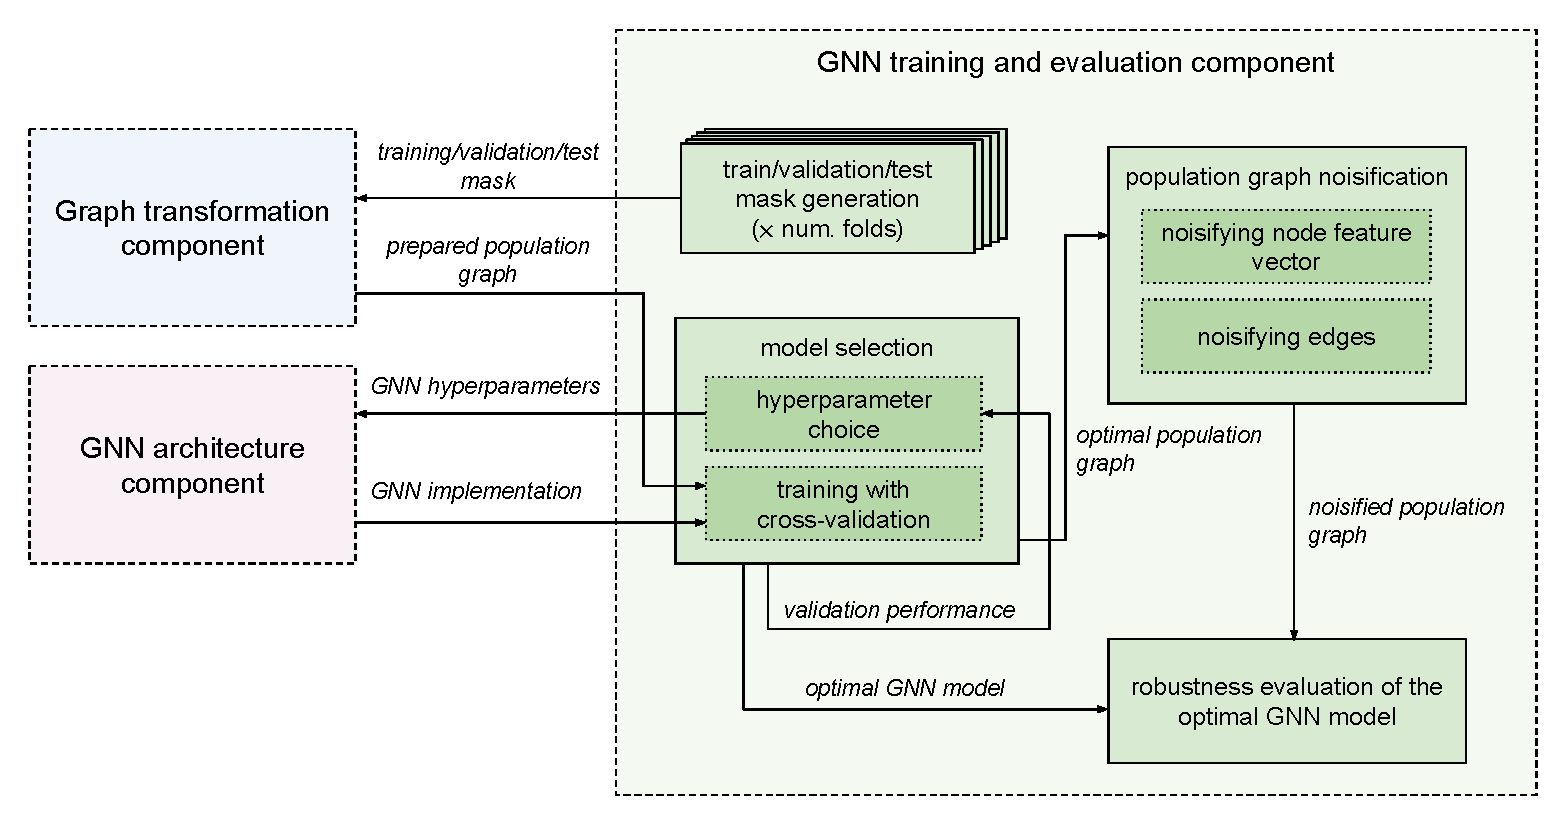
\includegraphics[width=\textwidth]{gnn_training_eval_component.pdf}
    \caption{GNN training and evaluation component.}\label{gnn-training-eval-component}
\end{figure}

\subsection{Model selection}
% Hyperparameter tuning, weights and biases

The brain age modelling task is challenging because of a vast combination of possible population graph and GNN hyperparameter choices. First, there is a choice of a neuroimaging modality combination for population graph node features (from functional, structural, and quality control data). Second, there are at least 32 combinations of possible non-imaging features used for similarity metrics (see Table~\ref{table:phenotype-features}), with each feature combination having a range of possible similarity thresholds. This does not account for the extension of using arbitrary linear combinations of non-imaging features for a similarity metric, and the fact that the UKB has over 760 more features that could potentially be included in similarity computation. Third, having fixed the population graph parameters, \texttt{BrainGNN} is in theory unlimited in its design and parameterisation possibilities (Table~\ref{table:braingnn}). Fourth, having fixed population graph and GNN hyperparameters, there are additional hyperparameters related to GNN training, such as the number of epochs and learning rate.

Having considered this, this section discusses further the motivation and reasoning behind most of the hyperparameter constraints and the training method. The full list of hyperparameter ranges that have been searched is included in Listing~\ref{listing:sweep-config}. 

\subsubsection{Memory constraints}
\label{section:memory}
% Tiago:  I won't get to the evaluation section today. It will be important to have in some part of your discussion the challenges of memory. That this is one big bottleneck in this type of analysis that needs to be tackled in the future. In case you don't mention this already

In the brain age estimation task with population graphs, the entire population graph containing node neuroimaging features, edges, GNN model training parameters and intermediate training states must be stored in memory at the same time. In addition, the population graph cannot be split into smaller independent batches since all nodes of the graph must be updated in a single training step, and it would be a non-trivial task to keep track of the edges and other interactions between the batches.

As a result, many hyperparameter combinations cause the model to run into memory issues. In practice, the models were limited to up to 8 gigabytes of GPU memory. This motivated the following hyperparameter constraints:

\begin{enumerate}
    \item \textit{Excluding functional data modality}. From preliminary experiments, using only functional and quality control data resulted in a poor graph neural network performance for the brain age estimation task. This is supported by the literature, such as the work of Niu et al.~\cite{niu2019improved}, which concluded that features derived from functional data were either not useful or even had a negative effect on predictive power, while structural features (particularly grey matter volume) were the most useful. Most importantly, functional data modality has over 70,000 features per subject (compared to 1,084 features for all remaining modalities combined), which results in an explosion in parameters for small estimated gain in performance. 
    
    Dimensionality reduction is possible, but from experience in the Data Science unit of assessment, cutting out half of the low-variance principal components can even worsen the predictive power and training time of the model instead of improving it. 
    
    While the functional data modality and dimensionality reduction technique were implemented~– indeed the goal of the pipeline was to support \textit{flexibility} to construct any population graph if needed (requirement R2, see Section~\ref{section:requirements-analysis}) – they were not used in training.
    \item \textit{Fixing the model size to a small set of shallow networks with a small number of units}. The learning rates were decreased and number of epochs increased to compensate for the smaller number of training parameters. The exact architecture is provided in Listing~\ref{listing:sweep-config}.
    \item \textit{Fixing the set of possible similarity feature sets and simlarity thresholds}. The default mode of averaging the feature-wise scores was used instead of arbitrary linear combinations, because, having no domain-specific knowledge of the relative importance of different confounders, this was the most non-informative, unbiased choice. From running some initial models, the feasible similarity thresholds have been all above 0.6, with even 0.7 or 0.8 often causing memory issues. This additionally motivated the use of as many non-imaging features as possible. \texttt{SEX} was always included in the feature sets because it is known to be an important confounder, significantly affecting the volume of the brain and sometimes even requiring a separate model for every sex~\cite{kaufmann2019}. The full list of population graphs tested can be found in Listing~\ref{listing:sweep-config}.
\end{enumerate}

\subsubsection{Hyperparameter tuning}
The hyperparameters were tuned using the Bayesian optimisation strategy provided by the \textit{Weights~\& Biases} (\texttt{wandb})~\cite{wandb} machine learning tracking and optimisation framework. Given the initial distributions of hyperparameters that should be searched (see Listing~\ref{listing:sweep-config}) and a command-line script that accepts hyperparameter combinations as arguments, \texttt{wandb} automatically selects the next set of hyperparameters that it believes is the most likely to improve a given performance metric. The choice of hyperparameters is based on both the initial hyperparameter distribution and the feedback from previously attempted values. For more information on Bayesian hyperparameter optimisation see Snoek et al.~\cite{snoek2012practical}.

Unlike in other hyperparameter tuning techniques such as grid search, Bayesian optimisation can use hyperparameter distributions defined over all real values in a given range. Consequently, hyperparameter search cannot be exhaustive and there is no obvious stopping point. In this project, hyperparameter tuning was run on each of the architectures until the models seemed to converge to similar performance with only marginal or no improvements as more hyperparameter combinations were tried. In general, this meant at least 100 hyperparameter combinations per GNN architecture, each hyperparameter combination trained five times for each cross-validation fold (see the next section), amounting to close to two weeks of total GPU compute time.

\subsubsection{Training procedure}
\label{section:training-procedure}

Before running the model selection and hyperparameter tuning procedure, the dataset is split into 90\% training/validation, and 10\% hold-out test set, stratifying by subject age and sex (as features that are the most likely to affect the brain age prediction). The test set is never used in training and hyperparameter tuning, and is only looked at during the evaluation procedure after the best hyperparameters for each of GCN and GAT have been selected (as indicated by the box at the bottom right in Figure~\ref{gnn-training-eval-component}). The subjects in the test set correspond to the \texttt{test\_mask} field of the population graph data structure as discussed in Table~\ref{table:population-graph} and Section~\ref{setting-training-masks}. While it is common to have multiple test sets (in techniques such as nested cross validation), this project does not use it because of the high computational cost and because the dataset is much larger than a typical brain imaging dataset (below 1,000 samples~\cite{parisot2018disease, cole2018brain} and often even less than 100 samples~\cite{franke2019ten}).

The remaining data is used for hyperparameter tuning. Each hyperparameter combination is trained using a stratified five-fold \textit{cross-validation}: the training/validation dataset is split into five folds with 90\% training and 10\% validation subjects, again stratifying by age and sex. These correspond to \texttt{train\_mask} and \texttt{validation\_mask} of the population graph data structure. This model selection strategy to a large extent follows the one in Raschka~\cite{raschka2018model}, Section 3.7.

The summary of the above steps is shown in Figure~\ref{gnn-training-eval-component}: the data splits are visualised with a set of different training/validation/test masks at the top left corner of the GNN training and evaluation component (all of them having the same test mask but different training and validation masks). The masks of each fold are used to transform the graph (in the graph transformation component), and for each fold the prepared population graph is trained on a GNN implementation with a given set of hyperparameters (as suggested by the \texttt{wandb} framework). The optimal GNN model and population graph hyperparameters are selected based on which hyperparameter combination gives the smallest mean squared error (MSE), averaged over the validation sets of each fold. MSE was chosen as the standard loss function used in regression tasks.

To prevent overfitting and optimise the training procedure, for every fold the models are trained with \textit{early stopping}: while validation loss itself is not used to update the parameters, the training stops as validation loss begins to increase with decreasing training loss (indicating overfitting on training data). At this point the weights are reverted back to when the validation loss was the smallest. In this project, the models are trained for at least 1,000 epochs and stopped early if MSE does not decrease by at least 0.005 over 100 consecutive iterations. 

As the hyperparameter tuning converges, the most promising model for each of the \texttt{BrainGCN} and \texttt{BrainGAT} architectures is selected to be tested on the hold-out test set. The metrics most commonly used in the literature for evaluating performance for the brain age (or any other regression) task~\cite{pervaiz2020optimising, niu2019improved} are Pearson's correlation $r$ and coefficient of determination $r^2$ (which will be further discussed in Section~\ref{section:evaluation-metrics}).

\subsection{Robustness measurement}
\label{section:implementation-robustness}

The proposed \textit{extension} for the training and evaluation component was to evaluate the robustness of the GNN models to the noise in the population graph, measured by the rate of performance drop with increasing noise. In this project, robustness is evaluated in two ways, testing for two different effects of noise: one of them associated with the noisy neuroimaging data, and the other with the population graph representation of the dataset.

MRI data can be very noisy~\cite{pervaiz2020optimising,niu2019improved}, and most neuroimaging preprocessing pipelines (such as the ones used for UKB dataset) use various techniques to remove noise caused by subject head motion, image distortion and other factors~\cite{glasser2013minimal}. This does not eliminate all noise, however, which motivates the development of models that could correct for those errors. 
%Intuitively, since the GNN architectures account for the features and labels of the node's neighbourhood when predicting some response variable, incorporating features of less noisy neighbours could improve the prediction for a noisy node. 
To test how the model performance changes with noise, increasing proportions of nodes could be corrupted. One way to do this would be to add Gaussian noise, but this leaves it unclear how to choose the optimal noise amplitude. A more aggressive way would be to corrupt the nodes completely by, for example, permuting their features.

Another advantage of using the population graph (rather than treating every subject as an independent example) is that the associations between subjects (captured through graph edges and defined by subject similarities) incorporate additional non-imaging information which could improve the predictions and account for confounding effects. To test whether the model relies on edge information, some fraction of edges that should have been present in the population graph could be removed, observing the change in model performance. 


\section{Repository overview}
% The repository overview should be around one page in length and should describe the high-level structure of the source code found in your source code Repository; ... could be implemented as a table with folders/file names and the functionality implemented in those files

The repository follows the structure of the five key project components shown in Figure~\ref{pipeline-overview}. Its overview is presented in Table~\ref{table:repository-overview}.


\begin{center}
    \small
    \begin{longtable}[]{p{0.25\textwidth}p{0.3\textwidth}p{0.4\textwidth}}
        \caption{Repository overview.}\label{table:repository-overview}\\
        \hline \textbf{Component} & \textbf{Filename} & \textbf{Notes} \\
        \hline
        \endfirsthead
        \multicolumn{3}{c}%
        {\tablename\ \thetable\ -- \textit{Continued from previous page}} \\
        \hline
        \textbf{Component} & \textbf{Filename} & \textbf{Notes} \\
        \hline
        \endhead
        \hline \multicolumn{3}{r}{\textit{Continued on next page}} \\
        \endfoot
        \hline
        \endlastfoot
% \begin{table}[]
%     \small
%     \begin{tabular}{p{0.25\textwidth}p{0.3\textwidth}p{0.4\textwidth}}
%         \hline
%     \textbf{Component} & \textbf{Filename} & \textbf{Notes} \\  \hline
    UKB preprocessing 
            & \texttt{phenotype.py} & Contains enumeration of non-imaging features, mappings of non-imaging feature names to their UKB codes. \\
            & \texttt{ukb\_preprocess.py} & Functionality described in Section~\ref{section:ukb-preprocessing}. \\
            & \texttt{ukb\_preprocess\_test.py} &  Tests for similarity matrix code. \\ \hline
    Graph construction
            & \texttt{graph\_construct.py} &Functionality described in Section~\ref{section:graph-construction}.\\
            & \texttt{graph\_construct\_test.py} & Tests for example population graph correctness. \\ \hline
    Graph transformation
            & \texttt{graph\_transform.py} & Functionality described in Section~\ref{section:graph-transformation}.\\ \hline
            % & \texttt{ukb\_preprocess\_test.py} &  \\   
    GNN architectures
            & \texttt{brain\_gnn.py} & Implementation of \texttt{BrainGNN} and extending classes \texttt{BrainGAT}, \texttt{BrainGCN} (Section~\ref{section:gnn-architecture}).\\ \hline
            % & \texttt{ukb\_preprocess\_test.py} &  \\   
    GNN training
            & \texttt{brain\_gnn\_evaluate.py} & Population graph noisification and robustness measurement procedure (Section~\ref{section:gnn-train-evaluate}). \\
            & \texttt{brain\_gnn\_train.py} & Cross-validation training procedure (Section~\ref{section:gnn-train-evaluate}). \\
            & \texttt{wandb\_sweep.yaml} & Initial hyperparameter distributions used by \texttt{wandb} (Listing~\ref{listing:sweep-config}). \\
            & \texttt{wandb\_train.py} & Command line script used by \texttt{wandb} to automatically test new hyperparameters. \\
    % \end{tabular}
    % \end{table}
\end{longtable}
\end{center}